\subsection{Sprint 2: 05.03 \textendash 18.03.2026}\label{subsec:sprint-2}

\subsubsection{Sprint Planning 2: 05.03.2026}\label{subsubsec:sprint-planning-2}

The current state of the project roadmap is shown in the following screenshot~\ref{fig:roadmap-sprint-planning-2}.

\begin{table}[H]
    \centering
    \begin{tabularx}{\textwidth}{l l X}
		\toprule
        \textbf{Week} & \textbf{Responsible} & \textbf{Task} \\
        \midrule
        Week 1 & Lukas & Configuration management implementation \\
        Week 1 & Frank & Research and comparison of frameworks \\
        Week 1 & Team & \gls{AI} workshop on Thursday and writing of the related issues \\
        Week 2 & Team & \gls{AI} research and evaluation \\
        Week 2 & Team & Preparation and pitch of the project deliverables \\
        \bottomrule
    \end{tabularx}
    \caption{Sprint Planning 2}
    \label{tab:sprint-planning-2}
\end{table}

\begin{figure}[H]
    \centering
    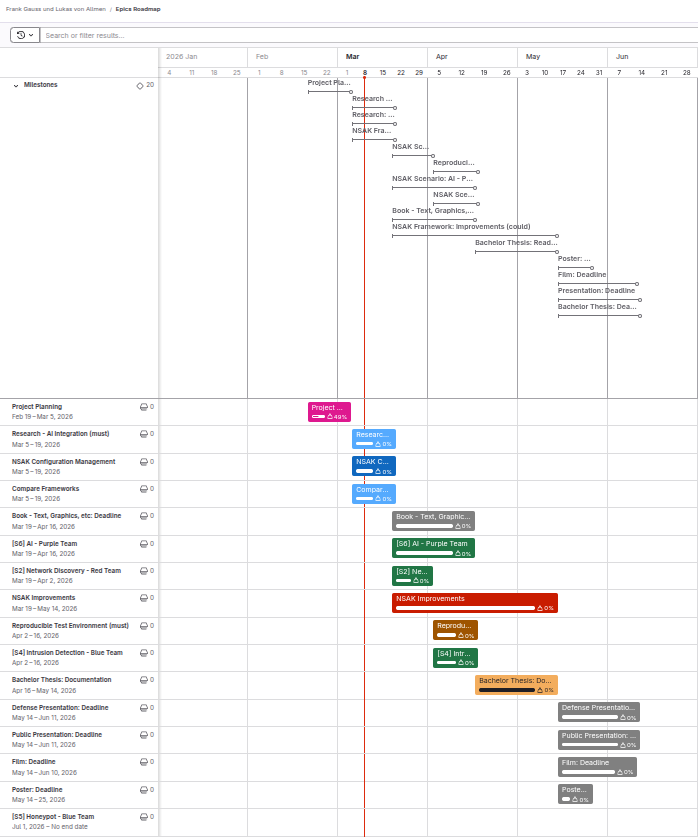
\includegraphics[width=1.0\linewidth]{../assets/screenshots/project_management/sprint_2/roadmap_sprint_planning_2}
    \caption{Roadmap Sprint Planning 2}
    \label{fig:roadmap-sprint-planning-2}
\end{figure}

\subsubsection{Sprint Review 2: 19.03.2026}\label{subsubsec:sprint-review-2}

We got some helpful inputs related to both milestones from the tutor and expert in the checkpoint meeting~\ref{subsec:checkpoint-meeting-3} earlier this day.
We decided to still consider the milestone to be successfully reached as the planned work package and deliverables were finalized and presented.
The resulting follow-up tasks are planned for the next week and as a consequence we will hold the next sprint planning~\ref{subsubsec:sprint-planning-3} a week later than planned.
All issues were reviewed and moved to the \enquote{Done} column in preparation for the next sprint.
It must be noted that the burnup and burndown charts are not really representative, as the project team often reviews and closes the tickets at the end of the sprint.

\paragraph{Milestone Review: Compare Frameworks}\label{par:milestone-review-compare-framework}

The Compare Frameworks~\ref{subsubsec:milestone-research-compare-frameworks} milestone is completed as illustrated in~\ref{fig:milestone-description-and-charts-framework-comparison]}.

\begin{figure}[H]
    \centering
    
\includegraphics[width=1.0\linewidth]{../assets/screenshots/project_management/sprint_2/milestone_framework_comparison_charts}
    \caption{Milestone Description and Charts: Compare Frameworks}
    \label{fig:milestone-description-and-charts-framework-comparison]}
\end{figure}

\paragraph{Milestone Review: Configuration Management}\label{par:milestone-review-configuration-management}

The burnup and burndown charts below~\ref{fig:milestone-description-and-charts-configuration-management]} are showing that the milestone Configuration Management~\ref{subsubsec:milestone-configuration-management} is implemented as planned.

\begin{figure}[H]
    \centering
    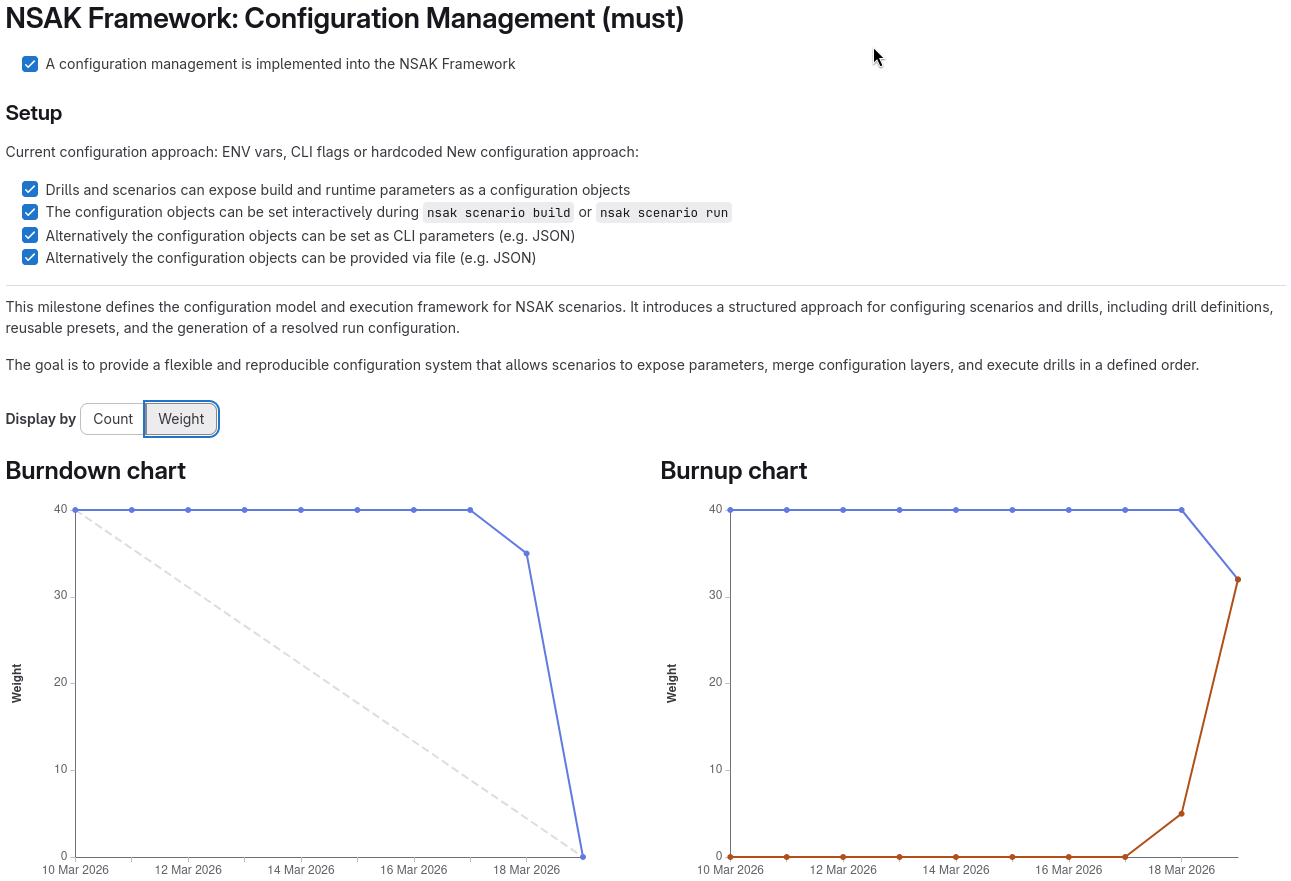
\includegraphics[width=1.0\linewidth]{../assets/screenshots/project_management/sprint_2/milestone_configuration_management_charts}
    \caption{Milestone Description and Charts: Configuration Management}
    \label{fig:milestone-description-and-charts-configuration-management]}
\end{figure}

\subsubsection{Sprint Retro 2: 19.03.2026}\label{subsubsec:sprint-retro-2}

This sprint retro was held in Microsoft Whiteboard as it provides simple templates, the result is illustrated in~\ref{fig:sprint-retro-2}.

\textbf{Key Takeaways:}

\begin{itemize}
    \item The long project planning phase greatly helped us with the projects overview and minimizes the planning needed for each sprint.
    \item The \enquote{focus weeks} really boosted the projects progress, and we are looking forward to the next \enquote{focus weeks}.
    \item Because we did not review tasks (\gls{QA}) on a regular basis, all this work needed to be done at the end of an iteration.
    \item Reviewing on a more regular basis would also lead to more accurate burndown and burnup charts.
\end{itemize}

\begin{figure}[H]
    \centering
    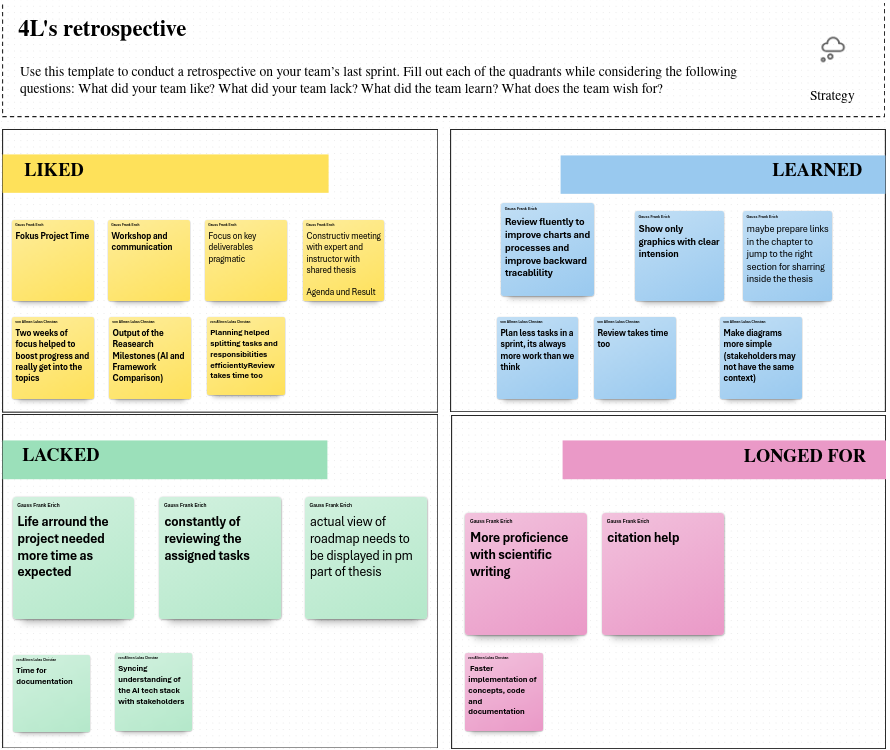
\includegraphics[width=1.0\linewidth]{../assets/screenshots/project_management/sprint_2/sprint_retro_2}
    \caption{Sprint Retro 2}
    \label{fig:sprint-retro-2}
\end{figure}
